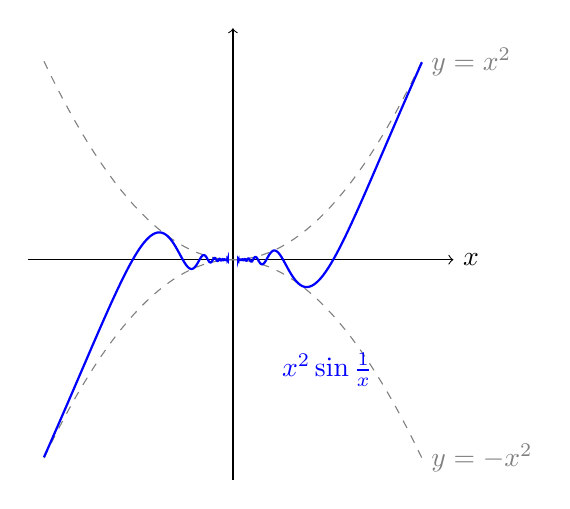
\begin{tikzpicture}[xscale=4, yscale=7]
  \draw[->] (-0.65,0) -- (0.7,0) node[right] {$x$};
  \draw[->] (0,-0.4) -- (0,0.42);
  \draw[gray, dashed, domain=-0.6:0.6, samples=60] plot (\x, {\x*\x}) node[right] {$y=x^2$};
  \draw[gray, dashed, domain=-0.6:0.6, samples=60] plot (\x, {-\x*\x}) node[right] {$y=-x^2$};
  \draw[blue, thick, domain=1.667:60, samples=1500, variable=\u] plot ({1/\u}, {sin(deg(\u))/(\u*\u)});
  \draw[blue, thick, domain=1.667:60, samples=1500, variable=\u] plot ({-1/\u}, {-sin(deg(\u))/(\u*\u)});
  \node[blue] at (0.3,-0.2) {$x^2\sin\frac1x$};
\end{tikzpicture}
